\chapter{Dataset - European Cloud Cover }
%This chapter presents the developed methodology used in the compilation of the dataset. 
This section presents the developed algorithms necessary for the compilation of the dataset \acrfull{ecc}. It is pieced together from two sources, ERA5 reanalysis and METeosat second generation cloud mask.

Several candidate satellites were studied before arriving at the combination of datasets presented here. Spatiotemporal consistency and resolution was given high priority. 
The variable cloud mask is provided by many satellites, bringing valuable information in itself, but also for the retrieval of other variables restricted to cloud free conditions, such as humidity. The satellite product chosen for this project is the \acrfull{msg}. This satellite is in geostationary orbit, and has an exceptional temporal resolution, scans every 15min. Knowing that the average lifetime of a cloud is 60min or less, it seems like a reasonable choice (\cite{lohmann2016}, pp. 19). The finished dataset, described in detail below, is named \acrfull{ecc}.

\section{Domain}
For this project the geographical domain has been restricted to latitude, $\theta \in[30,50]$ and longitude $\phi \in [-15, 25]$. The resulting dimensions of the grid become $81\times161$ pixels. Figure \ref{fig:map} shows the region of Europe included in this dataset, covering the central Europe and north Africa.
\begin{figure}[h]
    \centering
    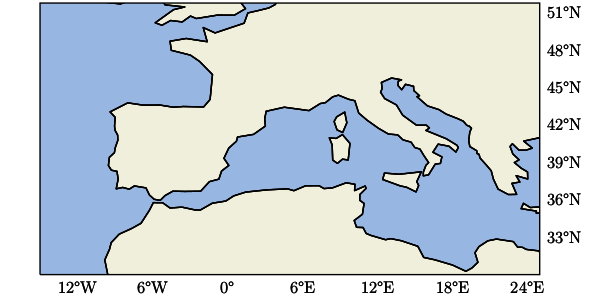
\includegraphics[scale = 1.0]{python_figs/Domain.png}
    \caption[Map over domain.]{Map showing the domain in the projection available in ECC. The region covers central Europe and north Africa.}
    \label{fig:map}
\end{figure}

\section{Physical basis of variable decision} \label{sec:ecc}
The overall goal is to investigate whether basic meteorological variables such as temperature, pressure and humidity are sufficient for prediction of cloud fractional cover with a reasonable accuracy. As discussed in Section \ref{sec:cloud_in_climate_system}, cloud dynamics is far more complicated than what can be describes by these variables. 

This is a \textit{proof of concept study} aimed to demonstrate the feasibility of using \acrshort{ai} to parametize \acrshort{cfc}. Employing data driven learning to represent cloud physics and dynamics in its full complexity requires measurements from technologies not yet invented. If they did exist, the computational cost would be enormous, and even then there would be no guarantee that the model performance would be state-of-the-art.
%Not feasible in the foreseeable future to incorporate all the effects of micro-physics at a sufficient accuracy. 

Macrophysics properties describes the cloud as a whole. Examples of such properties are base height, top height, thickness, fractional cover and regime also known as type. Microphysical processes are all mechanisms involving the particles making up a cloud. Examples of these variable are cloud condensation nuclei and droplet number concentrations (\cite{Grabowski2019ModelingBetter}). 

Precipitation formation and cloud optical thickness is affected by changes on a microphysical level. However, they are undeniably closely related to the macrophysical properties of the cloud. Imagine precipitation without a cloud fractional cover? 

Focusing on the macro-physical aspect of clouds its is reasonable to chose large-scale variables, for which reliable estimates are available from using reanalyse and other climate model, thereby ensuring that it is possible to build usable application of this in the future. 

The variables have been chosen because they are reliable (temperature and pressure) and/or cause the are essential in cloud formation (humidities). Other information may be present implicitly in these variables, being either surface variables or collected from the highest pressure level, the level closest to the surface. All variables are produced by ERA5. This section will give a brief introduction to their role in cloud formation. 

From the weather maps on the news, low and high pressure systems might be familiar terms. Low pressure systems are often associated with precipitation, while high pressure systems are associated with nice weather. Due to its spherical geometry the earth is not equally heated. Warmer air rises, this generates a low pressure at the surface. As the air rises the temperature decreases. Based on Equation \eqref{eq:clausius_clapeyron} its shown that, colder air can retain less vapour, enhancing the rate at which saturation is achieved. Under supersaturated conditions some of this vapour condenses, generating cloud water, forming a cloud, and occasionally precipitation. Summer is often associated with these convective motions generating cumulus type clouds. In presence of water at the surface, evaporation rates are also higher in a warmer climate. 

In areas of lower pressure the surrounding air will flow toward the low pressure centre in order to offset the pressure difference. Induced by Earths rotation the Coriolis effect force winds of low pressure system swirl counterclockwise north of the equator and clockwise south of the equator, causing an accumulation of air in the centre of low pressure system. Pushing it to higher altitudes in the atmosphere. A high pressure system exhibit the exact opposite behaviour, its swirls in the reverse direction, and the air flows from the centre. Diverging air masses cause sinking motions of parcels from higher in the atmosphere fill the space.
% air from higher in the atmosphere to sink and fill the space left.
% \textit{Air from higher in the atmosphere sinks down to fill the space left as air moves outward.} 
Winds transports the substances suspended in air, such as pollution and humidity.

The dataset includes both relative and specific humidity. Relative humidity is a measure of how much vapour the air contains, relative to much it can hold at that temperature. It is unitless, and ranges from 0 to 1. Conditions where relative humidity exceeds one are called supersaturated. Specific humidity is the ratio between mass of vapour and mass of air, with unit of $kg kg^{-1}$ (\cite{lohmann2016}, pp. 53-54). Whether the relative or specific humidity is the better predictor is not clear a priori. The data is gathered from the model level closest to the surface, at an altitude of 1000hPa (\cite{lohmann2016}, pp. 81-84). 

\section{Regridding scheme} \label{sec:remapping}
\begin{figure}
    \centering
    
    
\tdplotsetmaincoords{60}{110}
%
\pgfmathsetmacro{\rvec}{1.0}
\pgfmathsetmacro{\thetavec}{30}
\pgfmathsetmacro{\phivec}{60}

\pgfmathsetmacro{\deltathetavec}{40}
\pgfmathsetmacro{\deltaphivec}{80}

%
\begin{tikzpicture}[scale=5,tdplot_main_coords]
    \coordinate (O) at (0,0,0); % origo

    \coordinate (z) at (0, 0, 1.0); % origo
    %\draw[thin, <->] (1, 0.7, 1.16) -- (1, 0.52, 1.2) node[pos = 0.8, above right]{\Large $d\theta$};
    
    \draw[very thick,->] (0,0,0) -- (1.7, 0, 0) node[anchor=north east]{\Large $x$};
    \draw[very thick,->] (0,0,0) -- (0, 1.7, 0) node[anchor=north west]{\Large $y$};
    \draw[very thick,->] (0,0,0) -- (0, 0, 1.7) node[anchor=south]{\Large $z$};
    \shade[ball color = teal, opacity = 0.1] (0,0,0) circle [radius=\rvec];
    \draw (0,0,0) circle [radius=\rvec];
    
    \tdplotsetcoord{P}{\rvec}{\thetavec}{\phivec}
    \tdplotsetcoord{dP}{\rvec}{\deltathetavec}{\phivec}
    
    \tdplotsetcoord{G}{\rvec}{\thetavec}{\deltaphivec}
    \tdplotsetcoord{dG}{\rvec}{\deltathetavec}{\deltaphivec}

    \draw[very thick, color=teal, opacity = 0.3] (O) -- (G) node[above right]  {};
    \draw[very thick, color=teal, opacity = 0.6] (O) -- (dG) node[above right] {};    
    \draw[very thick, color=red, opacity = 0.6] (O) -- (P) node[above left]  {\Large $R$};
    \draw[very thick, color=teal, opacity = 0.6] (O) -- (dP) node[above right] {};
    
    \draw[dashed, color=teal] (O) -- (Pxy);
    \draw[dashed, color=teal] (dP) -- (Pxy);
    %\draw[dashed, color=red] (Pz) -- (Py);

    %\draw[dashed, color=red] (dP) -- (Pxy);
    
    \draw[very thick, color=red] (O) -- (Gxy) node[above right] {\Large $Rcos\theta$};
    \draw[dashed, color=teal] (dG) -- (Gxy);
    %\draw[dashed, color=black,looseness = 10, bend left] (z) -- (G)  node[pos = 0.6, above right] {\Large $Rsin\theta$};
    \draw[dashed, color=teal,looseness = 10, bend left] (z) -- (G);
    \draw[dashed, color=teal, bend right] (P) -- (z);
    
    
    \draw [very thick, color=blue] (\phivec:0.5)  arc (\phivec:\deltaphivec:0.5) node [below right, pos=0.3] {\Large $Rcos\theta d\phi$};

    
    %\tdplotdrawarc[tdplot_rotated_coords, ->]{(dP)}{.7}{(Pxy)}
    
    \draw[dashed, very thick, color=teal, fill = teal, opacity = 0.2] (P) -- (dP) -- (dG) -- (G) -- (P);
    \draw[dashed, very thick, color=teal] (P) -- (dP) -- (dG) -- (G) -- (P);
    \draw[very thick, color=blue] (dG) -- (G) node[pos = 0.5, above right] {\Large $Rd\theta$};
    \draw[dashed, color=teal] (dG) -- (G);    \tdplotdrawarc[]{(O)}{0.4}{0}{\phivec}{anchor=north}{\Large $\phi$}
    %\tdplotdrawarc{(O)}{0.2}{0}{\deltathetavec}{anchor=north}{$\theta$}

    \tdplotsetthetaplanecoords{\phivec};
    
    %\tdplotdrawarc[tdplot_rotated_coords]{(0,0,0)}{0.8}{0}%
        %{\thetavec}{anchor=south west}{\Large $\theta$};
    
    \tdplotdrawarc[tdplot_rotated_coords, pos = 0.01]{(0, 0.5, -0.3)}{0.45}{0.0}%
        {\thetavec}{anchor=south west}{\Large $\theta$};
    
    \tdplotdrawarc[tdplot_rotated_coords, pos = 0.5]{(0,0,0.2)}{0.26}{0}%
        {\thetavec}{anchor = south west,shift={(4mm,-5mm)}}{\Large $d\theta$};
        
    %\tdplotdrawarc[tdplot_rotated_coords, <->]{(0.1, 0.2, 0)}{.5}{0}{\thetavec}{anchor=east}{\Large $d\theta$}
    \shade[ball color=teal,tdplot_screen_coords,opacity=0.1] (O) circle[radius=\rvec];
    \foreach \X/\Y in {xy/z,yz/x,zx/y}
        {\begin{scope}[canvas is \X\space plane at \Y=\rvec]
         \fill circle[radius=1pt];
        \end{scope}}
    \end{tikzpicture}
    \caption{Properties of a square in spherical coordinates.}
    \label{fig:spherical_coords}
\end{figure}
Computing cloud fractions based on cloud mask requires a regridding scheme. Common schemes for solving similar tasks are mean, nearest neighbour or area weighting. For this particular task, since the pixels are of uneven size, the area weighted seemed most appropriate. This section will provided a step-by-step description of the necessary preprocessing done for the compilation of \acrshort{ecc}, transforming clouds masks provided in \textit{space-view} to cloud fractions on a uniform grid. \acrshort{eumetsat} doesn't provide suitable software to tackle this particular task (personal communication EUMETSAT staff). Building the dataset requires the implementations of this software.

Implementing this algorithm is twofold, first detection algorithms determining the contributing pixel to the particular cells in the other coordinate system. Secondly,  deriving the equation necessary for computing the area weighting. 

%The satellite retrievals are provided in a \textit{space-view} grid. 
Pixel-areas are computed using spherical coordinates. Figure \ref{fig:spherical_coords} shows how a square looks projected on to a sphere. Deriving the equation for computing the area of an square in spherical coordinates, requires integrating over changes in latitude, $\theta$ and longitude, $\phi$. The general expression for the area of a square in spherical coordinates, is given by the following integral. 
\begin{equation} \label{eq:sphere_integral}
    A = -R^2\int_{ \theta - \delta \theta }^{\theta + \delta \theta} \int_{ \phi - \delta \phi }^{\phi + \delta \phi} cos\left( \theta' \right) d\phi' d\theta'
\end{equation}
%This can be rewriting into, \textbf{needs indices $(i, j)$ ..?}
\begin{equation} \label{eq:sphere_finish}
    A \left( \theta, \phi, \delta \theta, \delta \phi   \right)= 2R^2 \left( sin\left( \theta + \delta \theta  \right) - sin\left(  \theta - \delta \theta  \right) \right) \delta \phi
\end{equation}
In relation to Figure \ref{fig:spherical_coords} $d \theta = 2 \delta \theta$, $d \phi = 2 \delta \phi$. Highlighting the parts necessary to compute an area, here $R=6378km$ denotes the distance to earth centre, $\theta$ the latitude and $\phi$ the longitude.

% Estimating the extent of the cell.
The coordinate information is provided as the latitude, $\theta$ (degrees north) and longitude, $\phi$ (degrees east) of the centre of the pixel. The area computation requires information about the extent of the cell, which requires some simplifications. The changes in longitude (latitude) at a certain pixel are estimated by the average distance to neighbouring points in the relevant directions. Approximation of $d\phi$ and $d\theta$ have been done based on the two-dimensional fields of latitude and longitude values according to the below equations \eqref{eq:app_lon} and  \eqref{eq:app_lat}. Let the horizontal extent of a pixel $(i,j)$ be determined by the the averaged distance between the longitude of neighbouring pixels, see Equation \eqref{eq:app_lon}. The same principles applies in the latitudinal direction, this version is shown in Equation \ref{eq:app_lat}.


\tdplotsetmaincoords{60}{110}
%
\pgfmathsetmacro{\rvec}{1.6}
\pgfmathsetmacro{\thetavec}{30}
\pgfmathsetmacro{\phivec}{60}

\pgfmathsetmacro{\deltathetavec}{40}
\pgfmathsetmacro{\deltaphivec}{80}

\begin{figure}
    \centering
    
    
\tdplotsetmaincoords{60}{110}
%
\pgfmathsetmacro{\rvec}{1.0}

\pgfmathsetmacro{\thetavec}{30}
\pgfmathsetmacro{\deltathetavec}{40}
\pgfmathsetmacro{\deltatwothetavec}{50}
\pgfmathsetmacro{\deltathreethetavec}{60}

\pgfmathsetmacro{\phivec}{-30}
\pgfmathsetmacro{\deltaphivec}{10}
\pgfmathsetmacro{\deltatwophivec}{50}
\pgfmathsetmacro{\deltathreephivec}{90}



\begin{tikzpicture}[scale=5,tdplot_main_coords, 
                    mycirc/.style={circle,fill=blue!20, minimum size=0.5cm}]

    %%%%%%%%%%%%%% Setting up axis and coordinate system.
    \coordinate (O) at (0,0,0); % origo
    \coordinate (z) at (0, 0, \rvec); % origo
    %\draw[thin, <->] (1, 0.7, 1.16) -- (1, 0.52, 1.2) node[pos = 0.8, above right]{\Large $d\theta$};
    \draw[very thick,->, opacity = 1.] (0,0,0) -- (1.7, 0, 0) node[anchor=north east]{\Large $x$};
    \draw[very thick,->,  opacity = 1.] (0,0,0) -- (0, 1.7, 0) node[anchor=north west]{\Large $y$};
    \draw[very thick,->,  opacity = 1.] (0,0,0) -- (0, 0, 1.7) node[anchor=south]{\Large $z$};
    \shade[ball color = teal, opacity = 0.1] (0,0,0) circle [radius=\rvec];
    \draw (0,0,0) circle [radius=\rvec];

    
    \tdplotsetcoord{a}{\rvec}{\deltathetavec}{\phivec}
    \tdplotsetcoord{b}{\rvec}{\deltatwothetavec}{\phivec}
    % Changeing the rightmost part 
    \tdplotsetcoord{c}{\rvec}{\deltathetavec-5}{\deltaphivec}
    \tdplotsetcoord{d}{\rvec}{\deltatwothetavec+5}{\deltaphivec}
    
    \draw[dashed, very thick, color=teal, fill = teal, opacity = 0.2] (a) -- (b) -- (d)-- (c) -- (a);
    \draw[dashed, very thick, color=teal] (a) -- (b) -- (d)-- (c) -- (a);

    \tdplotsetcoord{a}{\rvec}{\deltathetavec-5}{\deltaphivec}
    \tdplotsetcoord{b}{\rvec}{\deltatwothetavec+5}{\deltaphivec}
    \tdplotsetcoord{c}{\rvec}{\deltathetavec-10}{\deltatwophivec}
    \tdplotsetcoord{d}{\rvec}{\deltatwothetavec+10}{\deltatwophivec}
    
    \draw[dashed, very thick, color=teal, fill = teal, opacity = 0.2] (a) -- (b) -- (d)-- (c) -- (a);
    \draw[dashed, very thick, color=teal] (a) -- (b) -- (d)-- (c) -- (a);
        
    % First column
    %\node[draw] at (0, -2)  (c)     {C};
    %\node[draw] at (0.3, -0.25, 0.5) {$\phi_{(i,j-1)}$};
    %\node[draw, thick] at (0.5, 0.3, 0.65) {$\phi_{(i,j)})$};
    %\node[draw, thick] at (0.5, 0.73, 0.87) {$(i,j+1)$};
    \filldraw [teal, label=above:{$\phi_{(i,j-1)}$}]  (0.3, -0.25, 0.5) circle (1pt);
    \filldraw [teal, label=above:{$\phi_{(i,j-1)}$}]  (0.5, 0.3, 0.65)  circle (1pt);
    \filldraw [teal, label=above:{$\phi_{(i,j-1)}$}]  (0.5, 0.73, 0.87) circle (1pt);
    
    \tdplotsetcoord{a}{\rvec}{\deltathetavec-10}{\deltatwophivec}
    \tdplotsetcoord{b}{\rvec}{\deltatwothetavec+10}{\deltatwophivec}
    \tdplotsetcoord{c}{\rvec}{\deltathetavec-15}{\deltathreephivec}
    \tdplotsetcoord{d}{\rvec}{\deltatwothetavec+15}{\deltathreephivec}
    
    \draw[dashed, very thick, color=teal, fill = teal, opacity = 0.2] (a) -- (b) -- (d)-- (c) -- (a);
    \draw[dashed, very thick, color=teal] (a) -- (b) -- (d)-- (c) -- (a);
    
    \draw [decorate,decoration={brace, amplitude=12pt, mirror}, xshift=0pt, yshift=0pt]
    (0.3, -0.25, 0.1) -- (0.5, 0.83, 0.47) node [black,midway,xshift=0.2cm, yshift = -1.5cm, very thick] {\Large $\left| \phi_{i+1,j} - \phi_{i-1, j} \right| $};
    
    \draw [decorate,decoration={brace, amplitude=12pt}, xshift=0pt, yshift=0pt]
    (0.5, 0.3, 0.65) -- ((0.5, 0.5, 0.73) node [black,midway,xshift=0cm, yshift = 2.cm, very thick] {\Large $\delta \phi_{(i, j)}$};

    \tdplotsetthetaplanecoords{\phivec};
    \shade[ball color=teal,tdplot_screen_coords,opacity=0.2] (O) circle[radius=\rvec];
    \foreach \X/\Y in {xy/z,yz/x,zx/y}
        {\begin{scope}[canvas is \X\space plane at \Y=\rvec]
         \fill circle[radius=1pt];
        \end{scope}}
    \end{tikzpicture}
    
    \caption{Illustrating the relative size of three neighbouring pixels on a sphere in the \textit{space-view} grid provided by EUMETSAT. The following example explain the changes in longitude, $\phi$, varying in eastward direction, denoted $i$. The expression is shown in Equation \eqref{eq:app_lon}. 
    The same principles applies in the latitudinal direction, see Equation \eqref{eq:app_lat}.  }
    \label{fig:estimate_dlon}
\end{figure}

The cloud mask pixels are smallest at the nadir point, increasing in all other directions. Figure \ref{fig:estimate_dlon} shows an example of three neighbouring pixels where the apparent pixel size increases going eastward. This results in different distances from the centre to the right and left neighbour, to take advantage of the analytical expression derived in Equation \ref{fig:correct_area}, the extent is approximated by taking the average of the right and left distances. From Figure \ref{fig:estimate_dlon} it becomes evident that the squares resembles trapezium. As far as the author know, it doesn't exist a solution to a area of a trapezium in spherical coordinates, and its not clear if approximating this using using another numerical method.
%Since changes in degrees varies linearly this should not affect the extent of the cell. More than the error already present in the data. Det forklarer bare hvorfor buelengde ikke er nødvendig.
\begin{equation} \label{eq:app_lon}
    \delta \phi_{i,j} = \left| \frac{\phi_{i+1,j} - \phi_{i-1, j}}{4} \right|
\end{equation}
\begin{equation} \label{eq:app_lat}
    \delta \theta_{i,j} = \left| \frac{\theta_{i,j+1} - \theta_{i, j-1}}{4} \right|
\end{equation}

%\textbf{Present this as something that would be a minor correction.}
%A minor improvement, would be to derive the areas of trapezium in spherical coordinate, however this requires additional dependencies of 
%Failed to derive equations for trapezoidal shapes in spherical coordinate, therefore it never made sense to keep a different left, right, up and down extent. 

% Detecting which pixels that contribute to a cell.
Computing the area weighted average of cloud masks requires detecting the grid$_{\text{MGS}}$ contributing to the grid$_{\text{ERA5}}$ cell, and computing their area. The pixels are divided into five categories; \textit{centre}, \textit{left}, \textit{right}, \textit{up} and \textit{down boundary}. 

Let the subscripts denote the dataset pertaining to a particular grid. Grid$_{\text{MSG}}$ refers to the space-view grid of the \acrlong{msg} and grid$_{\text{ECC}}$ refers to the uniform grid originating from ERA5. It is worth noting that the grid$_{\text{ECC}}$ would be the same as grid$_{\text{ERA5}}$.
\begin{figure}
    \centering
    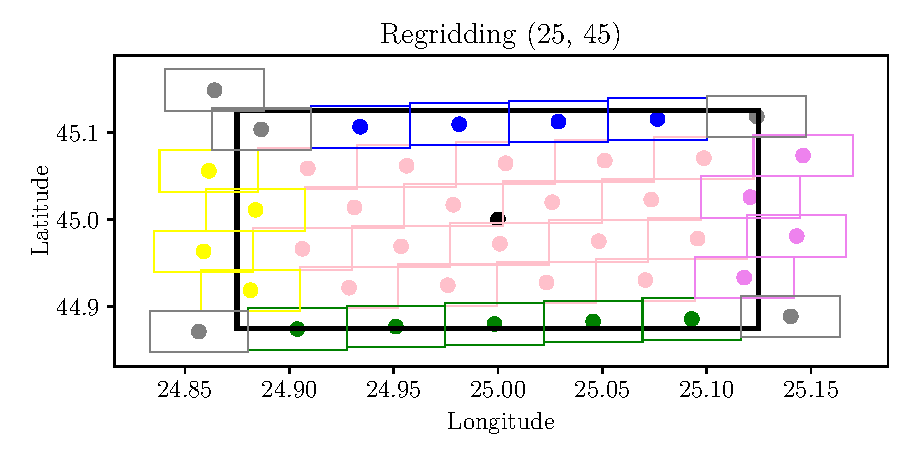
\includegraphics{python_figs/example_remapping_lat45_lon25.pdf}
    \caption{Remapping one cell, studying the number of pixels contributing to a cell. The pixels from satellite is classified into corner (grey), centre (pink), right (purple), left (yellow), down (green) and up (blue) } 
    \label{fig:pixels_contributing_to_cell.}
\end{figure}

\begin{equation} \label{eq:tot_area}
    A = \sum_{i=0}^{N} a_i
\end{equation}

\begin{equation} \label{eq:area_weighting}
    CF_{ECC} = \frac{1}{A} \sum_{i=0}^{N} a_i m_i
\end{equation}

One can easily prove that if all the mask $m_i = 1$ the cloud fraction, $CF_{ECC}=1$. This would not be true if the total area $A$, was determine by the extent of ECC/ERA5 cell. This explains why the overlap of neighbouring cell (see Figure \ref{fig:pixels_contributing_to_cell}) is not a cause for concern. The cloud fractions will not give unphysical values. The only affect worth mentioning is that some cloud mask, located at boundary pixels, contribute marginally more to the fraction than they should, but is in argued here that this is of little importance in the big picture.
% For the boundary categories we only include the contribution from within the cell. This is not actually a strict condition, including the entire area would still keep the fraction within its normal bounds of 0 and 1. However the boundary pixels would have a larger effect on the mean cloud cover since they contribute to several pixels. The footprint size effect on the distribution of cloud cover. For a large pixel size, and less contributing pixels we expect a higher number of grid-cells with close to 0 or 1 cloud amount. Since it alter the number of components you compute the average from.

% The cells in grid$_{\text{MGS}}$ contributing to a particular cell in grid$_{\text{ERA5}i,j}$ is fixed. In order to save computations on areas and detecting contribution pixels these are saved to \acrshort{json}-files. Made available in the the GitHub repository for supplementary material \href{https://github.com/hannasv/MS-suppl}{https://github.com/hannasv/MS-suppl}.

% Since the grid is constant, this is only done once and their indices and computed areas are stored in  Java Script Object Notification, json-files in the GitHub repository for supplementary material.
\begin{figure}[ht]
    \centering
    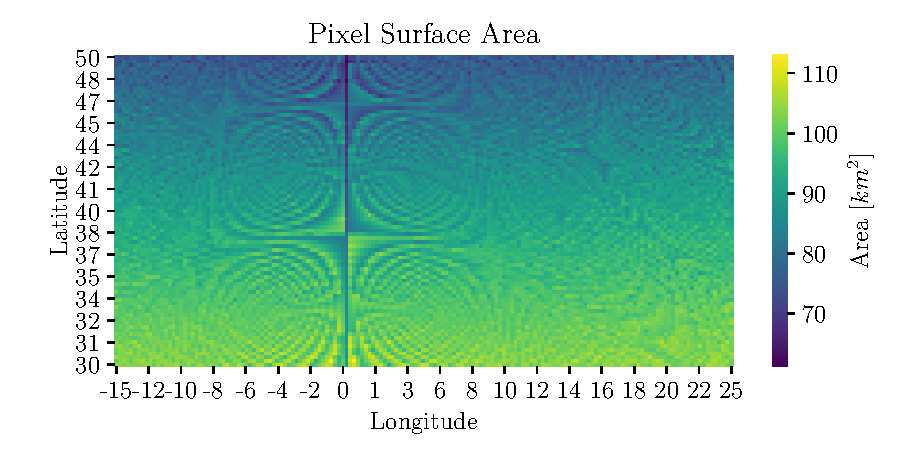
\includegraphics{python_figs/signal_area_pixel.pdf}
    \caption{Areas contribution to a pixel. This deacrease northward as illustrated in Figure \ref{fig:relative_size_neigbouring_pixels}.}
    \label{fig:area_pixel_signal}
\end{figure} 
\textbf{Comment this figure}
The cloud masks are provided from EUMETSAT in multiple formats. The \acrshort{grib}-format takes up less disk space. However this format doesn't provide coordinates for grid types such as space view. This information is available in \acrshort{netcdf}-format and is made available for the reader via the supplementary folder. All satellite images are provided using the same grid (personal correspondence with EUMETSAT staff). 

To recap, table \ref{tab:dataset_summary} contains a summary of the data used in the dataset.

\section{Testing regridding routine}
Since the different formats provide different rotations of the data. Recap the raw satelate images in \textit{grib} is provided east to west south to north. This is different from the postprocessed netcdf files providing data in the format east to west north to south, in other word, the rotation we are used to view the earth from space. Figure \ref{fig:visual_inspection_regridding} show the regridding of the raw data, clouds are illustrated in white, land mask in teal and ocean in purple. 
The original data is provided in four categories, land, ocea, cloud and off-earth disk. By regridded the raw data it quickly becomes apparent if the correct subsection of the dataset is used. 

Other meansures to ensure a correct regridding routine is tes

Equation \ref{eq:sphere_finish} is tested against CDO's the pixel area function, this is only uniform grids and the methods are compare based their computations of the areas in the ERA5 dataset. It is worth noting that the implementation is scaled by $R$ to be consistent with CDO code used in testing. This scaler factor is kept for the . Mutiplying by a large number, for so to divide by the same number provide no additional information, other than introducing additional numerical errors. 

\begin{figure}
    \centering
    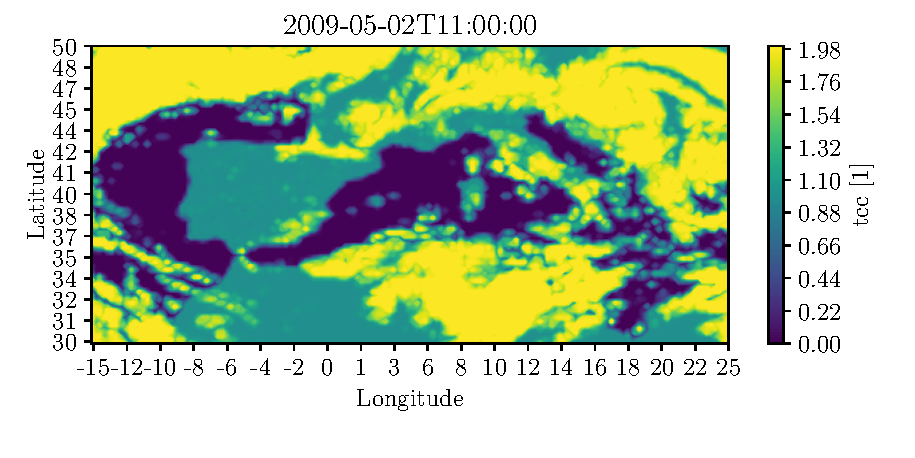
\includegraphics{python_figs/visual_regridding.pdf}
    \caption{Regridded the raw data including land sea pixels where there is no presence of clouds. A visual test of the regridded scheme, especially useful since different formats provide different rotation of the scan. TEAL - land, yellow is cloud and purple is ocean.}
    \label{fig:visual_inspection_regridding}
\end{figure}

\section{Missing Data} \label{sec:missing_values}
Missing valus is inevitable when working with observational data. 
\begin{figure}
    \centering
    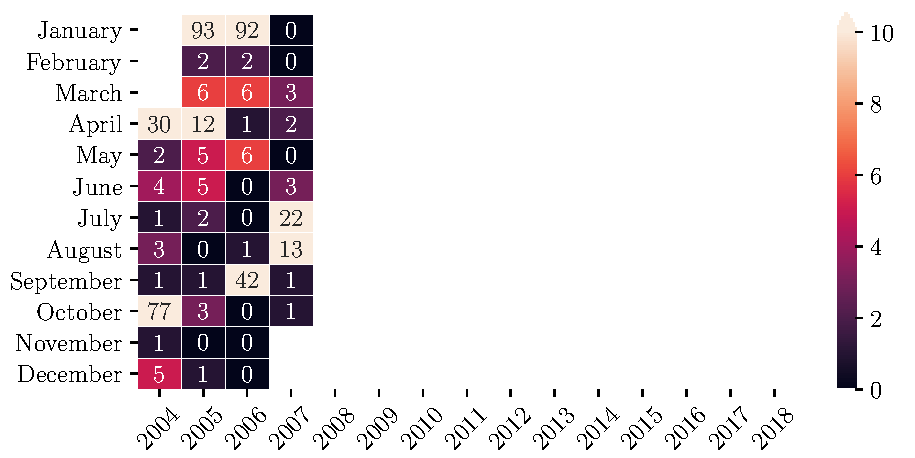
\includegraphics[scale = 1.0]{python_figs/heatmap_missing_values.pdf}
    \caption[Heatmap showing missing hours for all months or years.]{Heatmap displaying missing hours separated in month and years.}
    \label{fig:heatmap_missing_values}
\end{figure}
\begin{figure}
    \centering
    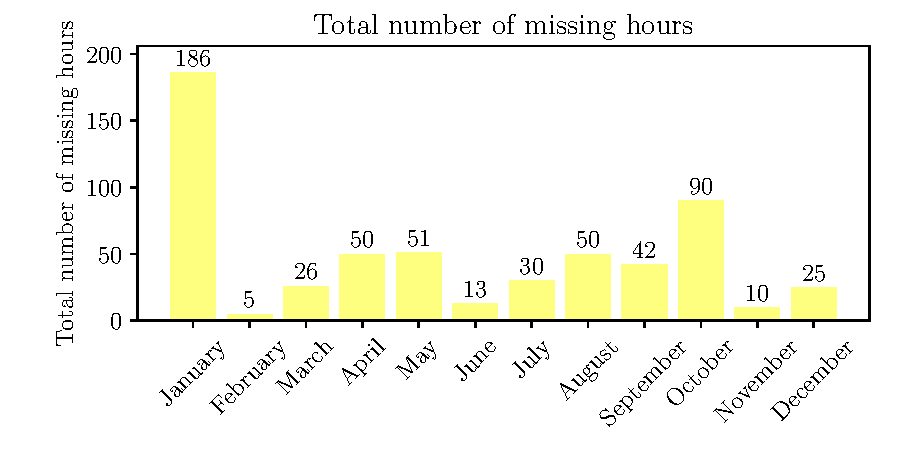
\includegraphics[scale = 1.0]{python_figs/heatmap_missing_values_monthly_sum.pdf}
    \caption{Barplot showing the monthly sum of missing values. This excludes the contribution from the periode of 2004 before the satellite was operational.}
    \label{fig:barplot_missing_values}
\end{figure}
he sensors fail to collect  measurements and data is missing. This can be either individual pixels or entire disks. In this project single NaN pixels are no pressing issue since they are remapped to fractions by using the area weighted mean. 


When the entire disks are missing, the closest time step available within the previous and trailing 45 minutes are chosen, if available. A summary of missing values per month in the data set is provided in Figure \ref{fig:heatmap_missing_values}. Aggregation of this missing values to month as provided in Figure \ref{fig:barplot_missing_values}. This is ment to illustrate any seasonal biases that might arise. This does not take into account the months before the satellite was operationalised in April of  2004. 

Manually generated datasets are prone to human error, especially since the user need to download individual timesteps to fill the gaps. The missing values was double checked, but there is no guarentee that a few additional timesteps is available. The workflow was as follows, the author downloaded the data, detect missing times and manually choose the closest time step available within the previous and trailing 45 minutes are chosen. 
In retrospect the, the downloading options should be wayed in when choosing data, this could avoid some frustration.

In some cases the data has been destroyed prior to archiving, and can never be recovered. The EUMETSAT staff has been made aware of this problem. Other issues arising in the process of downloading, requested data has entered infinity loop without being detected by EUMETSAT. The maximum limit of  pending request restricted to 20, slowed the process further down. One request can contain ca. 3.5 months of hourly data. 

As mentioned in Section \ref{sec:meteosat}, METEOSAT provide a two satellite system, occasionally both standby and the operational scan at the same time. To reduce the perturbations due to parallax of cloud, given a choice the operational satellite is chosen. In cases over technical failures, the standby scan is used, the scans are done from a different nominal position. The coordinate systems are the same, the standby scan is rectified to the position of the operational satellite before the data is provided. 
Before being rectified to the position of the position of the operational satellite. This introduces some complications related to the parallax. This becomes evident in comparison of simultaneous measurements for the operation and the standby METeosat satellites. There has been no effort in quatifing this parallax, beyond checking that retrival from the same timestap of different satellites are not identical. Adjusting for this could be moved into further work. Like reclassifiyng isolated pixels in AR results.

\section{Masks} \label{sec:mask}
The land sea masks are regridded from the HTAP-masks provided by \acrfull{metno}.  In its original format the HTAP masks have a $0.1^o$ resolution and global coverage, not including the polar regions. These are re-gridded to a suitable resolution of $0.25^o$ using functionality available in PyAEROCOM (\href{https://pyaerocom.met.no/}{https://pyaerocom.met.no/}). A python toolbox developed within the \acrfull{aerocom} project, storing only the domain relevant, available in the project supplementary repository. 
\begin{figure}
    \centering
    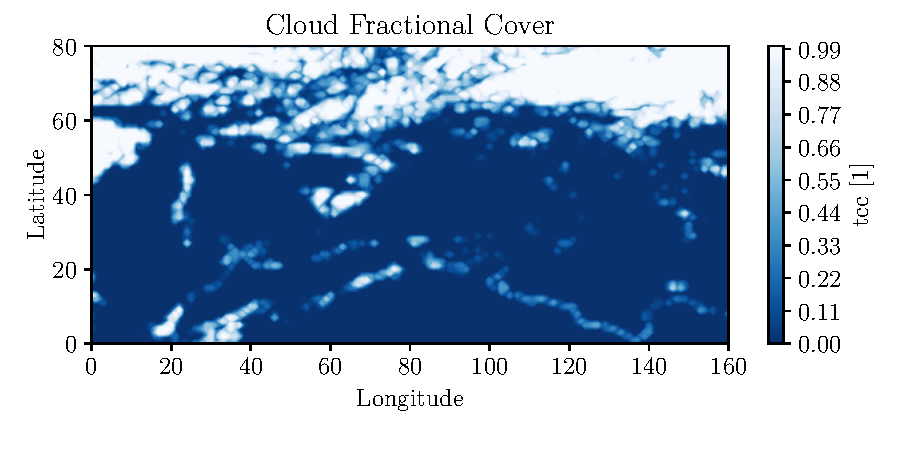
\includegraphics{python_figs/example_artefact.pdf}
    \caption[Artefact in European Cloud Cover dataset.]{Result from regridding, shows the artefact. Snapshop of artefact that is present in the dataset, ECC. The frequency of occurrence is currently unknown. \textbf{Plan to use the filter on every hour, storing the signal and plotting it in a histogram.}}
    \label{fig:example_artefact}
\end{figure}
\begin{figure}
    \centering
    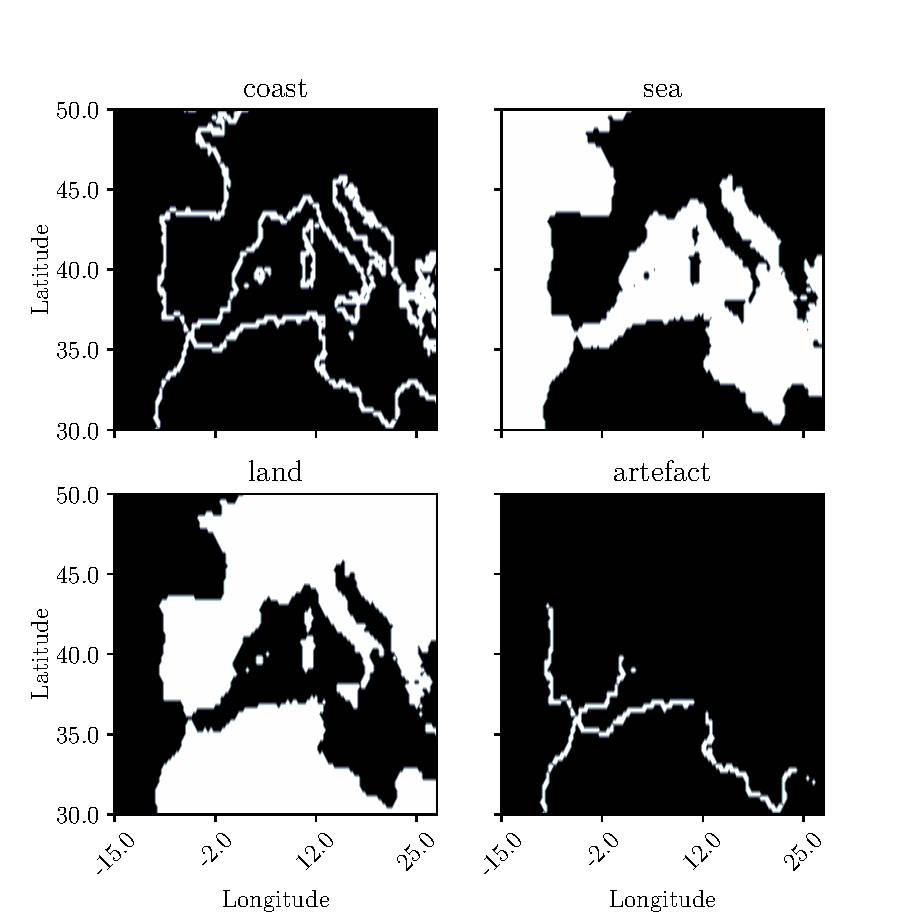
\includegraphics{python_figs/filters.pdf}
    \caption{Figure shows all filters, in white, available in the python package ``sciclouds''.}
    \label{fig:filters_subplot}
\end{figure}


Filters available \textit{land}, \textit{sea}, \textit{coastline} and \textit{artefact}. The coastline is defined to be all pixels that are not 100\% either land or sea. For land pixels, coastline pixels exceeding a 50\% threshold are included, the other pixels are regarded at the sea, argue that this is acceptable since this pixels at a level of at least 50\% most like sufficiently affected by maritime conditions that it is reasonable to classify them as sea pixels.

Defining the artefact according to equation, 
\begin{equation} \label{eq:artefact_condition}
    \theta + \frac{1}{3}\phi < 40
\end{equation}
Figure \ref{fig:filter_artefact} show the artefact detecting filter. To keep memory-requirements to a minimum only the parts of the filters relevant domain is stored in the supplementary material for this project.

The number of occurrences of this artefact seem to follow a normal distribution see Figure \ref{fig:signal_artefact}. Keep in min that there has been no attempts to distinguish this signal from when the entire region is cloudy. This could for instance be done by studiyng thie histograms from the ratio the artefact signal and land or no filter? The average cloud cover in the period is? 

\textbf{Signal artefact is not updated with all the cloud cover data.}

% Different approaches for detecting the artefact, separating the land, sea and coastline pixels. Filters to remove artefact in future. Can also use this compute statistics over land and ocean. Add land sea mask as subplot. 
Leaving the artefact in the data, its a project in itself to remove this without doing to much damage to the parts that are actually clouds that also produce a signal.

\section{Climatological Statistics}
%%% CORRELATION
\begin{figure}[ht]
    \centering
    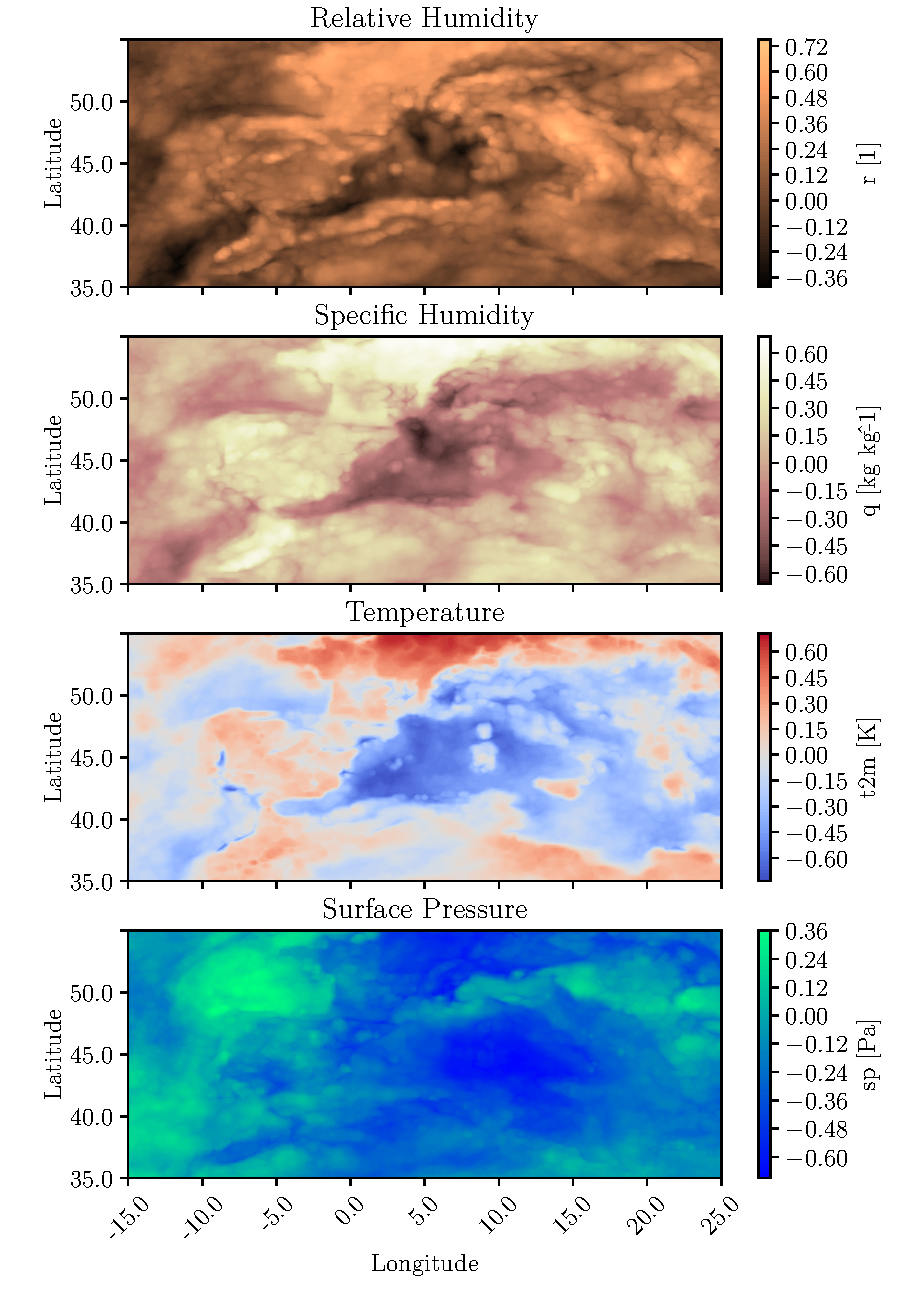
\includegraphics{python_figs/correlation_figure.pdf}
    \caption{Contour plot showing the correlation between environmental variables and cloud fractional cover. }
    \label{fig:correlation_tcc_vs_envio}
\end{figure}
Correlation describe how strong a pair of variables are linearly related. A positive correlation tells you that a increase in one variable results in a increase in the other. A negative correlation describes the opposite connection, implying that a increase in one variable cause a decrease in the other. Figure \ref{fig:correlation_tcc_vs_envio} show the linear correlation coefficient from pairs of cloud cover and environmental variables such as temperature, pressure, relative and specific humidity.
Keep in mind that the environmental values in this study is reanalysis variables. 

Pink illustrates negative correlation while green illustrates a positive correlation. Different patterns emerge from all variables, implying that they could be useful as predictors. Over land relative humidity is positively related to 
In the same region surface pressure is negatively correlated with cloud cover. This seems reasonable, since high pressure is often caused by sinking motions in the atmosphere and clouds are formed by rising motions. Over land in North Africa, Western Europe and in the Alps specific humidity is positive correlated to cloud cover and in eastern parts and above the ocean they are positively correlated. In most locations temperature is negatively correlated with cloud cover except in parts of the Alps, north coast of France and in north Africa. 
Dissuasion  --- Related to AR-model re

%%% BAR PLOT GLOBAL STATISTICS
\begin{figure}[ht]
    \centering
    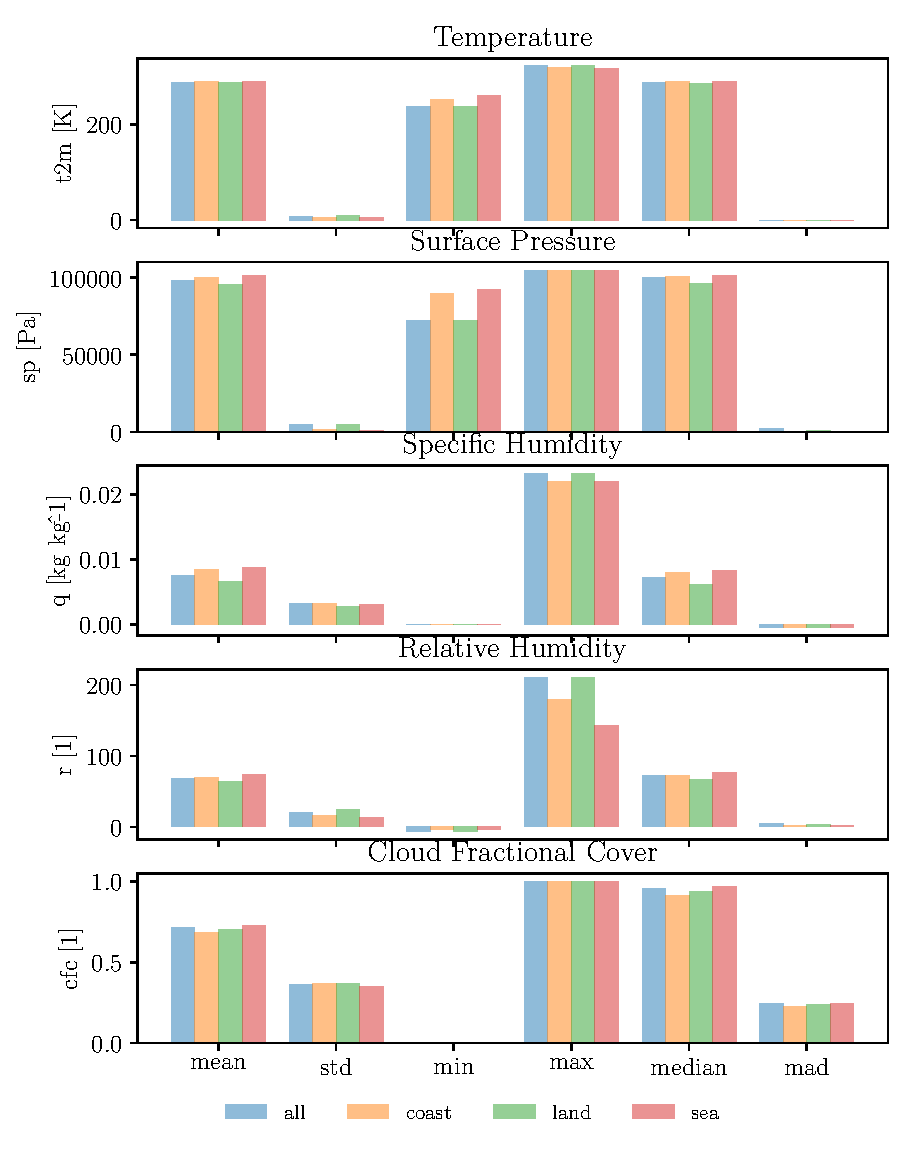
\includegraphics{python_figs/bar_plot_global_statistics_new_legend.pdf}
    \caption{Bar plot showing global statistics for different filters. \textbf{Notice the low std and mad. Can this be explained by the fact that they are generated by a model.}}
    \label{fig:bar_plot_global_stats}
\end{figure}
To study the statistical properties at different parts of the domain the filters shown in Figure \ref{fig:filters_subplot} was applied to the data before computing the statistical properties. Figure \ref{fig:bar_plot_global_stats} shows a barplot summarising the mean, standard deviation (std), min, max, median and mean absolute deviation (mad) for the five variables and four filters including the entire region. It becomes evident that there are differences between the different filter, however they are not ginormous.

%% CLOUD FRACTIONAL COVER
\begin{figure}[ht]
    \centering
    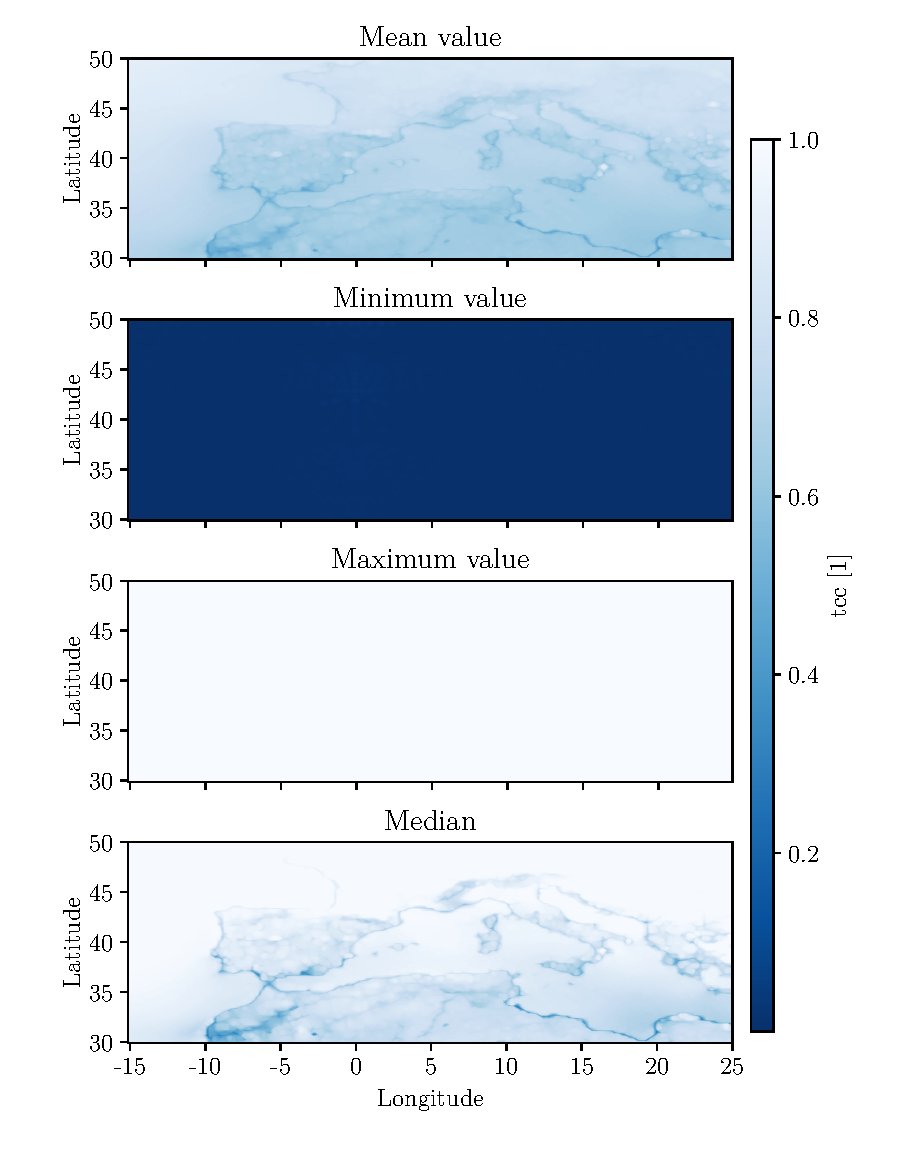
\includegraphics{python_figs/all_stat_variable_tcc.pdf}
    \caption{Contour plot showing the local (pixel) statistics for cloud fractional cover.}
    \label{fig:all_stats_tcc}
\end{figure}
Moving from top to bottom, the mean values show that on average the coastline have a lower cloud cover than the adjacent areas. This is supported by the bar plot (see Figure \ref{fig:bar_plot_global_stats}). From the minimum values of cloud cover it becomes evident that there is a  artefact present in the dataset. This is caused by the remapping routine. Figure X shows the patterns of magnitude of the areas contributing to a pixel. The max value is a one over the entire region, this tells you that at some point every pixel is cloudy. No suprises there. 
The standard deviation is higher over land, this is caused by larger variation in cloud cover in these regions. The median and mad show similar patterens, with lowest values along the coast.

Thought it is not exactly identical the same, the circular pattern centered around the median shown in the \ref{fig:area_pixel_signal} could be a possible explination of the minimum values in cloud cover. The presence of a artefact caused by the area-weighting regridding sheme.

%%%%%%%%%%%%%%%%%%%%%%%%%%%%%%%%%%% MONTHLY MEANS
\begin{figure}[ht]
    \centering
    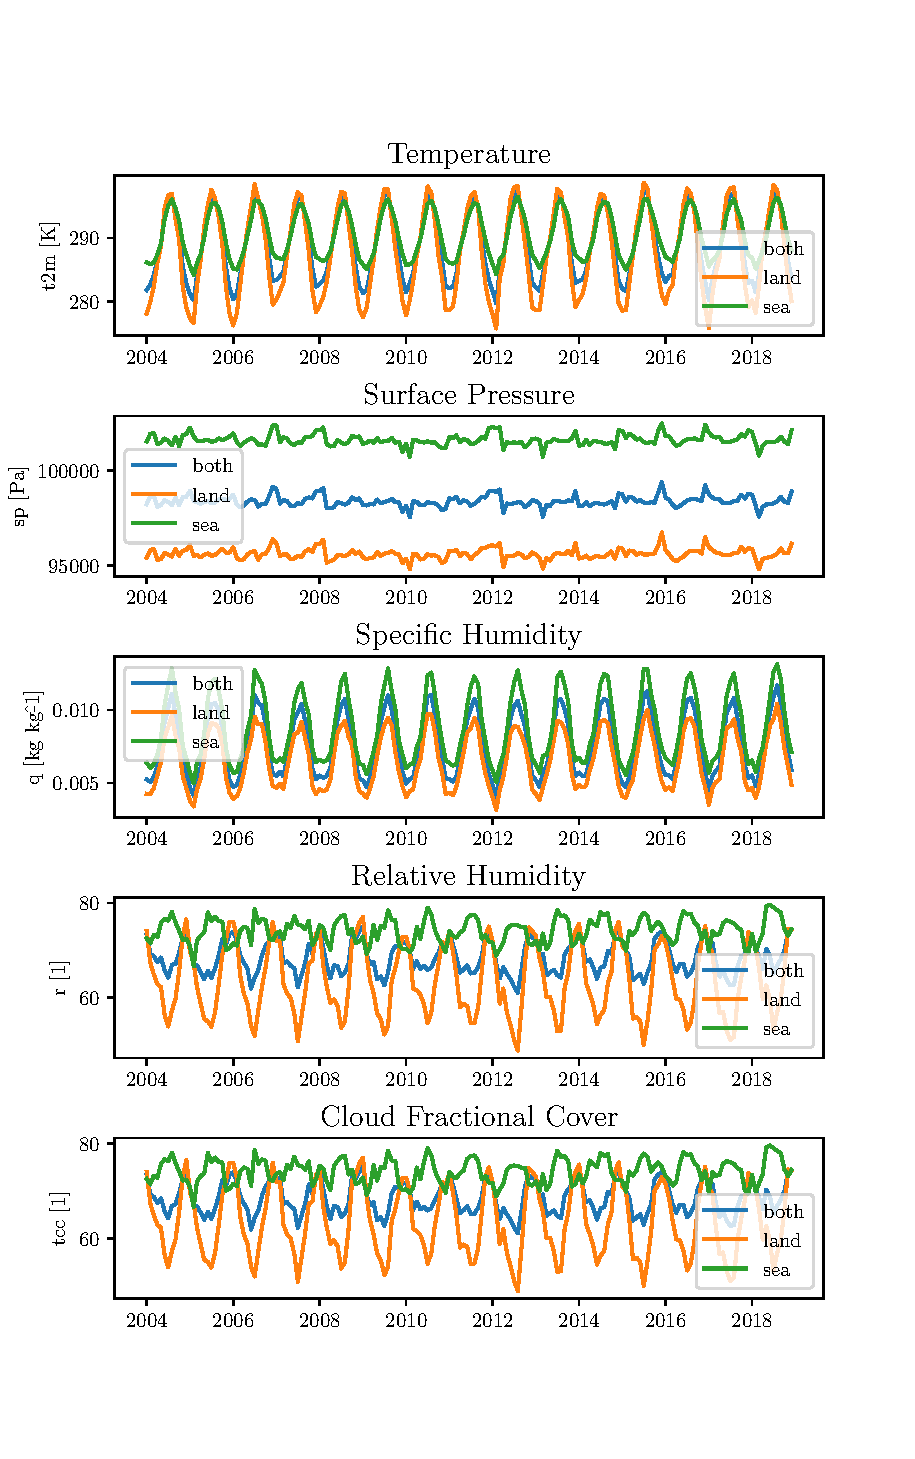
\includegraphics{python_figs/monthly_means.pdf}
    \caption{Spatially averaged monthly values. Filters are applied for land and sea.}
    \label{fig:monthly_mean_ts_vars}
\end{figure}
Figure \ref{fig:monthly_mean_ts_vars} shows the spatially averaged monthly mean values for all values. Seasonal effects and differences between land and ocean is evident among all variables.


Figure \ref{fig:random_week} shows the spatially averaged time series for the first week of August in 2012. It is ment to illustrate the relative strength of the signal feed to the input sequence. As a reference, the signal over land and ocean is provided. All variables display diurnal variations.

\begin{figure}[ht]
    \centering
    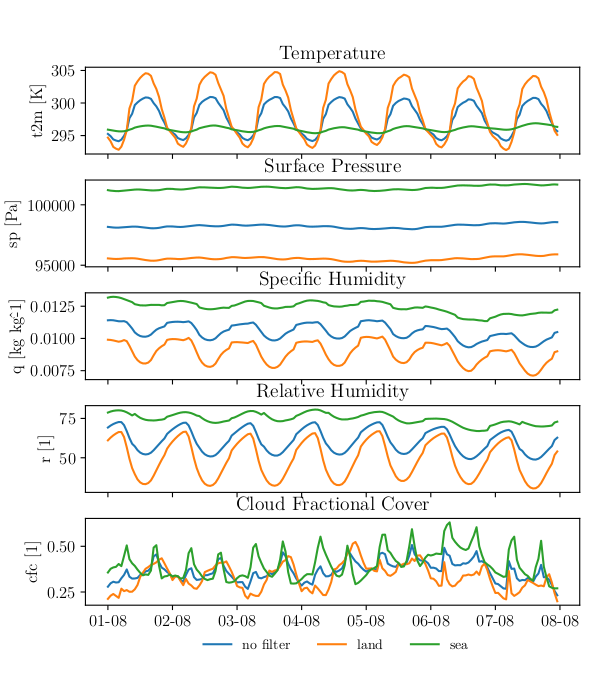
\includegraphics{python_figs/spatially_averaged_one_week_from_2012-08-01.png}
    \caption{Spatially averaged time series, the filters are applied for land and sea.}
    \label{fig:random_week}
\end{figure}
Figure % \ref{fig:temporally_averaged_data} 
shows the temporally averaged time series for all variables in the dataset. The topography is a clear factor, comparing this contour plot to Figure \ref{fig:map} the patterns are very similar. 

% Finished regriddidng files.
\section{Summary}
\acrshort{ecc} comprises of five variables collected from two sources; ERA5 and EUMETSAT. The resolution available in ERA5 was preserved, while remapping the cloud mask to cloud fractions. The final product consist of the variables temperature, pressure, cloud fraction, specific humidity and relative humidity, available hourly data on a $0.25^o$ uniform grid resolution in the period from April 2004 to December 2018. Cloud fractional cover (\acrshort{cfc}) is produced from area weighting cloud masks. These computations are described in \ref{sec:remapping}. The remaining variables are on their original format as provided by \acrfull{ecmwf}. A summary of the original sources of the dataset is given in Table \ref{tab:dataset_summary}. More details on ERA5 is available in Section \ref{sec:era5} and on Section \ref{sec:EUMETSAT_cloud_mask} for more information about cloud mask. 
\begin{table}[]
    \centering
    \resizebox{\textwidth}{!}{%
\begin{tabular}{c|c|c|c|c|}
\cline{2-5}
\multirow{4}{*}{}                                 & \multicolumn{2}{c|}{\textbf{ERA5}}                                                                                                   & \multicolumn{2}{c|}{\textbf{MSG2}}                                                                                                                \\ \cline{2-5} 
                                                  & \textbf{Type}                     & \textbf{Variables}                                                                               & \textbf{Type}                                                               & \textbf{Variables}                                                  \\ \cline{2-5} 
                                                  & Surface                           & \begin{tabular}[c]{@{}c@{}}2m Temperature\\ Surface pressure\end{tabular}                        & \multirow{2}{*}{Satelite retrival}                                          & \multirow{2}{*}{Cloud Mask}                                         \\ \cline{2-3}
                                                  & 1000 hPa                          & \begin{tabular}[c]{@{}c@{}}Relative Humidity\\ Specific Humidity\end{tabular}                    &                                                                             &                                                                     \\ \hline
\multicolumn{1}{|c|}{\textbf{Projection}}         & \multicolumn{2}{c|}{Uniform grid}                                                                                                    & \multicolumn{2}{c|}{Curve linear grid}                                                                                                            \\ \hline
\multicolumn{1}{|l|}{\textbf{Spatial resolution}} & \multicolumn{2}{c|}{$0.25^o$}                                                                                                        & \multicolumn{2}{c|}{-}                                                                                                                            \\ \hline
\multicolumn{1}{|c|}{\textbf{Output Frequencey}}  & \multicolumn{2}{c|}{Hourly}                                                                                                          & \multicolumn{2}{c|}{15 min}                                                                                                                       \\ \hline
\multicolumn{1}{|c|}{\textbf{Availability}}       & \multicolumn{2}{c|}{\begin{tabular}[c]{@{}c@{}}1979-onwards\\ Expected to be available from \\ 1950 some time in 2020.\end{tabular}} & \multicolumn{2}{c|}{2004-onward}                                                                                                                 \\ \hline
\multicolumn{1}{|c|}{\textbf{License}}           & \multicolumn{2}{c|}{\begin{tabular}[c]{@{}c@{}}Open Access. Need user \\ from Copernicus Data Storage.\end{tabular}}                  & \multicolumn{2}{c|}{\begin{tabular}[c]{@{}c@{}}Researcher Licences\\ to get 15min resolution.\\ Open access at \\ hourly resolution\end{tabular}} \\ \hline
\end{tabular}
}
\caption{Data description on the data present in the dataset ECC (European Cloud Cover). \textbf{Add projection as a column, Availability for download and the period of data.} There is a lot of work in combining the two datasets and processing it.}
\label{tab:dataset_summary}

\end{table}
%Fractional cloud cover is computed from the cloud mask product retrieved by the second generations METeosat satellites. You can read more about this data in section \ref{sec:meteosat}. For simplicity we will refer to this dataset as European Cloud Cover Dataset, ECC from now on. The visual comparison between raw satellite images and cloud amount seem to agree. The cloud fractional distribution also retain the same shape as ERA5 and MODIS 6.1 Terra in the period from 2004 to 2018. \textbf{kilde?}

%\textbf{Something is missing here -- a table?}

%\subsection{Licences and Downloading Data} \label{sec:downloading_data}
%Scripts for downloading the ERA5 data used in this thesis is available in the project GitHub on \href{https://github.com/hannasv/MS/tree/metos/downloading{\_}RA}{https://github.com/hannasv/MS/tree/metos/downloading{\_}RA}. However you will need to create a CDS-user. Follow the instructions on ECMWF homepages on \textit{how to download ERA5}. There are no scripts available for downloading METEOSAT data this is done using satellite retrievals at EUMETSATs Earth Observation Portal. Its freely available in hourly resolution. Scientist can apply for increased resolution up to 15min. Choose the cloud mask product in grb-format. By running \textbf{X - legg inn filnavn} you can generate your own files for regridding. The supplementary material only include the domain used in this thesis, because of GitHub has a maximum limit allowed for uploading. 
\tdplotsetmaincoords{60}{110}
%
\pgfmathsetmacro{\rvec}{1.6}
\pgfmathsetmacro{\thetavec}{30}
\pgfmathsetmacro{\phivec}{60}

\pgfmathsetmacro{\deltathetavec}{40}
\pgfmathsetmacro{\deltaphivec}{80}

\begin{figure}
    \centering
    
    
\tdplotsetmaincoords{60}{110}
%
\pgfmathsetmacro{\rvec}{1.0}

\pgfmathsetmacro{\thetavec}{30}
\pgfmathsetmacro{\deltathetavec}{40}
\pgfmathsetmacro{\deltatwothetavec}{50}
\pgfmathsetmacro{\deltathreethetavec}{60}

\pgfmathsetmacro{\phivec}{-30}
\pgfmathsetmacro{\deltaphivec}{10}
\pgfmathsetmacro{\deltatwophivec}{50}
\pgfmathsetmacro{\deltathreephivec}{90}

\begin{tikzpicture}[scale=5,tdplot_main_coords]

    %%%%%%%%%%%%%% Setting up axis and coordinate system.
    \coordinate (O) at (0,0,0); % origo
    \coordinate (z) at (0, 0, \rvec); % origo
    %\draw[thin, <->] (1, 0.7, 1.16) -- (1, 0.52, 1.2) node[pos = 0.8, above right]{\Large $d\theta$};
    \draw[very thick,->, opacity = 1.] (0,0,0) -- (1.7, 0, 0) node[anchor=north east]{\Large $x$};
    \draw[very thick,->,  opacity = 1.] (0,0,0) -- (0, 1.7, 0) node[anchor=north west]{\Large $y$};
    \draw[very thick,->,  opacity = 1.] (0,0,0) -- (0, 0, 1.7) node[anchor=south]{\Large $z$};
    \shade[ball color = teal, opacity = 0.1] (0,0,0) circle [radius=\rvec];
    \draw (0,0,0) circle [radius=\rvec];

    %%%%%%%%%%%%%%%%%%%%%%%%%%%% first column
    \tdplotsetcoord{P}{\rvec}{\thetavec}{\phivec}
    \tdplotsetcoord{dP}{\rvec}{\deltathetavec}{\phivec}
    \tdplotsetcoord{G}{\rvec}{\thetavec}{\deltaphivec}
    \tdplotsetcoord{dG}{\rvec}{\deltathetavec}{\deltaphivec}
    
    \draw[dashed, very thick, color=teal, fill = teal, opacity = 0.2] (P) -- (dP) -- (dG) -- (G) -- (P);
    \draw[dashed, very thick, color=teal] (P) -- (dP) -- (dG) -- (G) -- (P);
    
    \tdplotsetcoord{a}{\rvec}{\deltathetavec}{\phivec}
    \tdplotsetcoord{b}{\rvec}{\deltatwothetavec}{\phivec}
    \tdplotsetcoord{c}{\rvec}{\deltathetavec}{\deltaphivec}
    \tdplotsetcoord{d}{\rvec}{\deltatwothetavec}{\deltaphivec}
    
    \draw[dashed, very thick, color=teal, fill = teal, opacity = 0.2] (a) -- (b) -- (d)-- (c) -- (a);
    \draw[dashed, very thick, color=teal] (a) -- (b) -- (d)-- (c) -- (a);
    
    \tdplotsetcoord{e}{\rvec}{\deltatwothetavec}{\phivec}
    \tdplotsetcoord{f}{\rvec}{\deltathreethetavec}{\phivec}
    \tdplotsetcoord{g}{\rvec}{\deltatwothetavec}{\deltaphivec}
    \tdplotsetcoord{h}{\rvec}{\deltathreethetavec}{\deltaphivec}
    
    \draw[dashed, very thick, color=teal, fill = teal, opacity = 0.2] (e) -- (f) -- (h)-- (g) -- (e);
    \draw[dashed, very thick, color=teal] (e) -- (f) -- (h)-- (g) -- (e);

    %%%%%%%%%%%%%%%%%%%%%%%%%%%%%%%% second column
      
    \tdplotsetcoord{P}{\rvec}{\thetavec}{\deltaphivec}
    \tdplotsetcoord{dP}{\rvec}{\deltathetavec}{\deltaphivec}
    \tdplotsetcoord{G}{\rvec}{\thetavec}{\deltatwophivec}
    \tdplotsetcoord{dG}{\rvec}{\deltathetavec}{\deltatwophivec}
    
    \draw[dashed, very thick, color=teal, fill = teal, opacity = 0.2] (P) -- (dP) -- (dG) -- (G) -- (P);
    \draw[dashed, very thick, color=teal] (P) -- (dP) -- (dG) -- (G) -- (P);
  
      
    \tdplotsetcoord{a}{\rvec}{\deltathetavec}{\deltaphivec}
    \tdplotsetcoord{b}{\rvec}{\deltatwothetavec}{\deltaphivec}
    \tdplotsetcoord{c}{\rvec}{\deltathetavec}{\deltatwophivec}
    \tdplotsetcoord{d}{\rvec}{\deltatwothetavec}{\deltatwophivec}
    
    \draw[dashed, very thick, color=teal, fill = teal, opacity = 0.2] (a) -- (b) -- (d)-- (c) -- (a);
    \draw[dashed, very thick, color=teal] (a) -- (b) -- (d)-- (c) -- (a);
  
  
    \tdplotsetcoord{e}{\rvec}{\deltatwothetavec}{\deltaphivec}
    \tdplotsetcoord{f}{\rvec}{\deltathreethetavec}{\deltaphivec}
    \tdplotsetcoord{g}{\rvec}{\deltatwothetavec}{\deltatwophivec}
    \tdplotsetcoord{h}{\rvec}{\deltathreethetavec}{\deltatwophivec}
    
    \draw[dashed, very thick, color=teal, fill = teal, opacity = 0.2] (e) -- (f) -- (h)-- (g) -- (e);
    \draw[dashed, very thick, color=teal] (e) -- (f) -- (h)-- (g) -- (e);
    
    
    %%%%%%%%%%%%%%%%%%%%%%%%%%%%%%%% third column
    \tdplotsetcoord{P}{\rvec}{\thetavec}{\deltatwophivec}
    \tdplotsetcoord{dP}{\rvec}{\deltathetavec}{\deltatwophivec}
    \tdplotsetcoord{G}{\rvec}{\thetavec}{\deltathreephivec}
    \tdplotsetcoord{dG}{\rvec}{\deltathetavec}{\deltathreephivec}
    
    \draw[dashed, very thick, color=teal, fill = teal, opacity = 0.2] (P) -- (dP) -- (dG) -- (G) -- (P);
    \draw[dashed, very thick, color=teal] (P) -- (dP) -- (dG) -- (G) -- (P);
  
    \tdplotsetcoord{a}{\rvec}{\deltathetavec}{\deltatwophivec}
    \tdplotsetcoord{b}{\rvec}{\deltatwothetavec}{\deltatwophivec}
    \tdplotsetcoord{c}{\rvec}{\deltathetavec}{\deltathreephivec}
    \tdplotsetcoord{d}{\rvec}{\deltatwothetavec}{\deltathreephivec}
    
    \draw[dashed, very thick, color=teal, fill = teal, opacity = 0.2] (a) -- (b) -- (d)-- (c) -- (a);
    \draw[dashed, very thick, color=teal] (a) -- (b) -- (d)-- (c) -- (a);
  
    \tdplotsetcoord{e}{\rvec}{\deltatwothetavec}{\deltatwophivec}
    \tdplotsetcoord{f}{\rvec}{\deltathreethetavec}{\deltatwophivec}
    \tdplotsetcoord{g}{\rvec}{\deltatwothetavec}{\deltathreephivec}
    \tdplotsetcoord{h}{\rvec}{\deltathreethetavec}{\deltathreephivec}
    
    \draw[dashed, very thick, color=teal, fill = teal, opacity = 0.2] (e) -- (f) -- (h)-- (g) -- (e);
    \draw[dashed, very thick, color=teal] (e) -- (f) -- (h)-- (g) -- (e);
    
    %%%%%%%%%%%%%%%%%%%%%%%%%% Adding coordinate information

    % First column
    \draw[thick](0.3, -0.25, 0.5)node[scale=0.8, rotate = -15]{$(i,j-1)$};
    \draw[thick](0.3, -0.17, 0.7)node[scale=0.8, rotate = -15]{$(i+1,j-1)$};
    \draw[thick](0.3, -0.3, 0.3)node[scale=0.8, rotate = -15]{$(i-1,j-1)$};

    % Second column
    \draw[thick](0.5, 0.3, 0.65)node[scale=0.8, rotate = 5]{$(i,j)$};
    \draw[thick](0.5, 0.3, 0.85)node[scale=0.8, rotate = 5]{$(i+1,j)$};
    \draw[thick](0.5, 0.3, 0.45)node[scale=0.8, rotate = 5]{$(i-1,j)$};
    
    % Third column
    \draw[thick](0.5, 0.73, 0.87)node[scale=0.8, rotate = 35]{$(i,j+1)$};
    \draw[thick](0.5, 0.8, 0.7)node[scale=0.8, rotate = 35]{$(i-1,j+1)$};

    \draw[thick](0.05, 0.45, 0.73)node[scale=0.8, rotate = 35]{$(i+1,j+1)$};

    \tdplotsetthetaplanecoords{\phivec};
    \shade[ball color=teal,tdplot_screen_coords,opacity=0.1] (O) circle[radius=\rvec];
    \foreach \X/\Y in {xy/z,yz/x,zx/y}
        {\begin{scope}[canvas is \X\space plane at \Y=\rvec]
         \fill circle[radius=1pt];
        \end{scope}}
    \end{tikzpicture}
    
    \caption{Sketch to illustrated the relative size of neighbouring pixels in uniform grid of ECC, projected onto spherical coordinates. The areas of pixels in a uniform grid decrease poleward.}
    \label{fig:relative_size_neigbouring_pixels}
\end{figure}